\begin{figure*}[t]
\centering
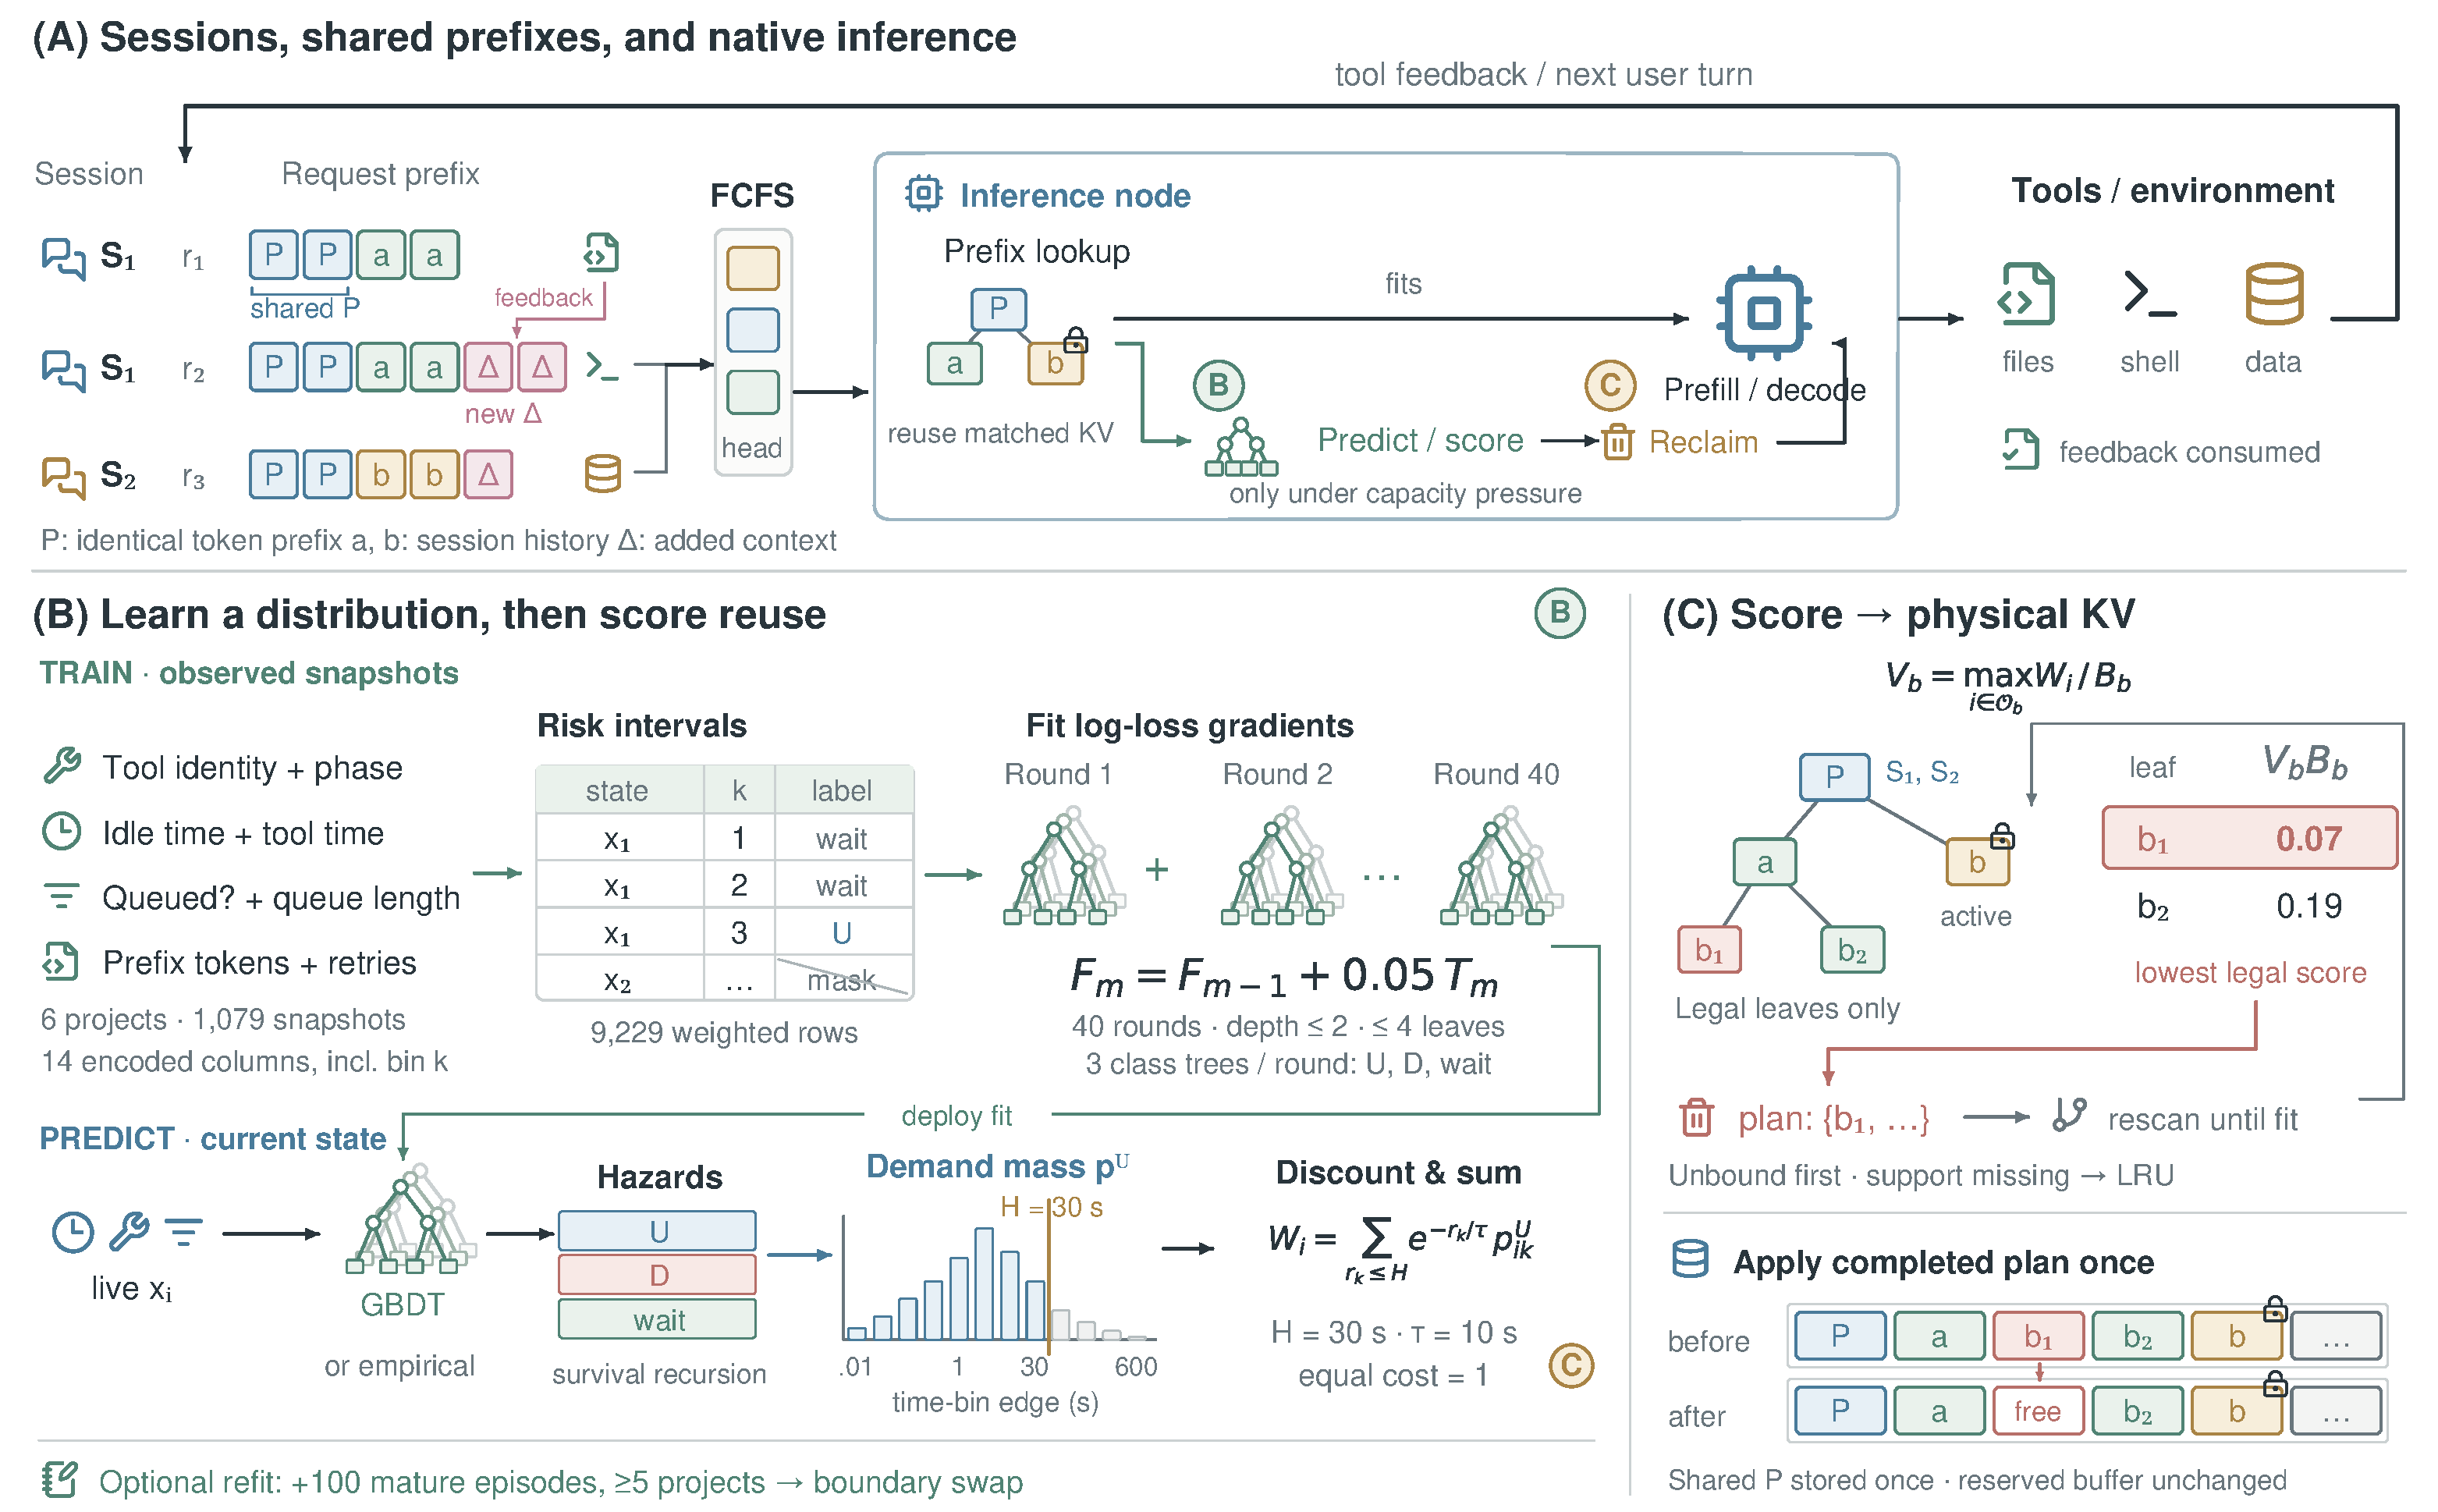
\includegraphics[width=\textwidth]{leasepath_isca_v3_assets/figures/leasepath_method_overview.pdf}
\caption{LeasePath workflow. \textbf{(A)} Shared prefixes, overlapping tools, and FCFS inference. \textbf{(B)} Observed snapshots train interval classifiers; predicted demand masses become discounted retention scores. \textbf{(C)} Legal leaves form a logical plan before native reclamation. Counts describe the initial fit; histories, example rows, trees, bars, and equal-size-block scores are schematic.}
\Description{A: three request histories include a common identical prefix P, session-specific suffixes, and added context. They enter FCFS native inference; matching prefix KV is reused, while capacity pressure invokes prediction/scoring B and reclamation C. Real tools feed results into later requests. B: tool identity, phase, idle/tool elapsed time, readiness, queue length, prefix tokens, retries, missingness, and interval index form fourteen encoded columns. The initial fit has 1079 snapshots from six development projects and 9229 weighted risk-interval rows. Waiting intervals, observed events, and censoring masks define the targets. Forty boosting rounds use three class trees per round, learning rate 0.05, depth at most two and at most four leaves. Hazards become unconditional demand masses through survival recursion; equal-cost discounted scoring uses H thirty seconds and tau ten seconds. Optional refits require one hundred additional mature episodes from at least five projects, then a boundary swap. C: maximum owner score per payload byte ranks legal unprotected leaves. Unbound leaves go first; unsupported scores use LRU. Logical removals and candidate rescans build a complete plan before it is applied once to native KV. Shared prefixes occupy one physical copy. Deletion frees used cells without shrinking the reserved buffer. The tree shapes, request histories, bars, and candidate values are schematic.}
\label{fig:method-overview}
\end{figure*}
